\documentclass[generalized_symmetry.tex]{subfiles}
\setcounter{chapter}{4}
\begin{document}

\chapter{高次元の非可逆対称性}
高次元の非可逆対称性は比較的新しい話題で、現在も盛んに研究が進んでいる分野です。高次元の非可逆対称性の系統的な調べ方はまだありません。いくつかの例が知られているだけです。高次元の非可逆対称性の発見の仕方にはいくつかあるのですが、ここでは2つの方法を紹介します。
\begin{itemize}
  \item 高次ゲージ化(higher gauging)
  \item 半空間ゲージ化(half-space gauging)
\end{itemize}
後者は\ref{sec:KWdefect}節でKramers-Wannier双対性の欠陥を作るのに用いた方法の高次元版です。名前を見て分かるとおり、両方とも「ゲージ化」の方法ですので、まずは高次形式対称性のゲージ化について説明します。

\section{高次形式対称性のゲージ化}
$G$を有限アーベル群とし、$\Tcal$を$d$次元の場の理論で$p$形式$G$対称性($G^{(p)}$対称性)っを持つものとします。$X$を$d$次元の向きのついた閉リーマン多様体とします。$K$を$X$の単体分割とします。
この単体分割を利用して$G^{(p)}$対称性に対する背景ゲージ場を$A\in Z^{p+1}(X;G)$として導入します。この背景ゲージ場のもとでの分配関数を$Z_{\Tcal}(A)$と表します。

\subsection{ゲージ化した理論の分配関数}

$Z_{\Tcal}(A)$がアノマリーが無い場合、つまり$Z_{\Tcal}(A+\delta \lambda)=Z_{\Tcal}(A)$が成り立ち、しかも単体分割のしかた$K$に依存しない場合を考えます。このとき、ゲージ化した理論$\Tcal/G^{(p)}$を考えることができます。その分配関数$Z_{\Tcal/G^{(p)}}(A)$はすべてのゲージ場の配位について足し合わせることで得られます。
\begin{align}
  Z_{\Tcal/G^{(p)}} = \frac{1}{\mathrm{Vol}} \sum_{a \in Z^{p+1}(X;G)} Z_{\Tcal}(a)
  \label{gaugingcochain}
\end{align}
$\mathrm{Vol}$はゲージ体積であり、ゲージ変換でつながるようなゲージ場の配位を何回も数えている分を割っておくものです。

ゲージ体積について少し考えてみます。以下、式を短くするために$C^p(K,G)$のことを引数を省略して単に$C^p$と書くことにします。素朴にはゲージ変換のパラメーター$\lambda \in C^{p}$の数なので$1/\mathrm{Vol} = 1/|C^p|$と考えられます。しかし、$\lambda \in C^p$がすべて独立なゲージ変換のパラメーターではなく、$\lambda\in C^p$と$\lambda+d\sigma$, $\sigma \in C^{p-1}$は同じゲージ変換を表しますので、$|C^{p-1}|$で割る必要があります。しかし、話はこれで終わりではなく、$\sigma \in C^{p-1}$もすべて独立なパラメーターではなく……と続けていく必要があります。最終的には
\begin{align}
  \frac{1}{\mathrm{Vol}} =
  \begin{cases}
    \frac{|C^{p-1}||C^{p-3}|\dots 1}{|C^p||C^{p-2}|\dots |C^0|}  & (p \text{ が偶数のとき}) \\
    \frac{|C^{p-1}||C^{p-3}|\dots |C^0|}{|C^p||C^{p-2}|\dots 1}  & (p \text{ が奇数のとき})  
  \end{cases}
  \label{gaugevolcochain}
\end{align}
となります。

文献等ではこれらはコチェイン$C^*$の言葉ではなくてコホモロジーの言葉で書いてあることも多いと思います。それについてここで説明します。まず、$H^{p+1}=Z^{p+1}/B^{p+1}$なので、
\begin{align}
  \sum_{a \in Z^{p+1}(X;G)} Z_{\Tcal}(a)=|B^{p+1}|\sum_{a \in H^{p+1}} Z_{\Tcal}(a)\label{gaugingtemp}
\end{align}
となります。また、完全系列(前の写像の像が次の写像の核になるような系列)
\begin{align}
  0 \to Z^{p} \overset{i}{\to} C^{p} \overset{\delta}{\to} B^{p} \overset{\delta}{\to} 0 
\end{align}
を考えることができます。ここで$i$は包含写像です。この完全系列から
\begin{align}
  B^{p+1}=C^{p}/Z^{p}
\end{align}
であることが分かります。これらの関係を用いると
\begin{align}
  |B^{p+1}|&=\frac{|C^{p}|}{|Z^{p}|}=\frac{|C^{p}|}{|H^p||B^p|}=\frac{|C^{p}||B^p|}{|H^p||C^{p-1}|}=\dots\\
  &=\frac{|C^{p}||C^{p-2}|\dots }{|C^{p-1}||C^{p-3}|\dots}\times
  \frac{|H^{p-1}||H^{p-3}|\dots }{|H^p||H^{p-2}|\dots } 
\end{align}
となります。これを\eqref{gaugingtemp}に代入し、さらに\eqref{gaugevolcochain}、\eqref{gaugevolcochain}を用いると
\begin{align}
  Z_{\Tcal/G^{(p)}} = \frac{|H^{p-1}||H^{p-3}|\dots }{|H^p||H^{p-2}|\dots } \sum_{a \in H^{p+1}} Z_{\Tcal}(a)
\end{align}
という表式を得ます。この他に重力に関する局所項を入れることもできます。

\subsection{双対対称性}
2次元の場合と同様に有限アーベル群$p$形式対称性をゲージ化した理論$\Tcal/G^{(p)}$には双対対称性が存在します。これについて見ていくことにしましょう。

双対対称性のトポロジカル欠陥はWilsonサーフェスと呼ばれる演算子です。これは$\rho\in \hat{G}$(1次元ユニタリー表現)つまり$\rho:G\to \U(1)$(準同型)、$c \in Z_{p+1}(K,\Zb)$として
\begin{align}
  W_{\rho}(c) = \rho\left(\int_{c} a\right)
\end{align}
を挿入することです。この欠陥は$p+1$次元ですから、余次元は$d-p-1$次元になります。つまりこれは$(d-p-2)$形式対称性のトポロジカル欠陥になります。まとめると、
\begin{emphasize}
  $\Tcal/G^{(p)}$は$\hat{G}^{(d-p-2)}$対称性を持つ。
\end{emphasize}
ということが言えます。

これをさらに詳しく見るために$G=\Zb_N$の場合に限って考えます。この場合、$q=d-p-2$としてWilsonループの情報は$B \in H^{q+1}$で表されます。この背景での分配関数は
\begin{align}
  Z_{\Tcal/G^{(p)}}(B) = \frac{|H^{p-1}||H^{p-3}|\dots }{|H^p||H^{p-2}|\dots } \sum_{a \in H^{p+1}} Z_{\Tcal}(a) \exp\left(\frac{2\pi i}{N}\int_{X} B\cupp a\right)
\end{align}
となります。ゲージ化すると、だいたい分配関数はFourier変換したようなものになります。

この$\hat{G}^{q}$対称性をゲージ化した理論$\Tcal/G^{p}/\hat{G}^q$を考えます。この分配関数は
\begin{align}
  Z_{\Tcal/G^{(p)}/\hat{G}^{(q)}} =& \frac{|H^{q-1}||H^{q-3}|\dots }{|H^q||H^{q-2}|\dots } \sum_{c \in H^{p+1}} Z_{\Tcal/\hat{G}^{q}}(b)\notag\\
  =&\frac{|H^{q-1}||H^{q-3}|\dots }{|H^q||H^{q-2}|\dots } \sum_{b \in H^{q+1}} \frac{|H^{p-1}||H^{p-3}|\dots }{|H^p||H^{p-2}|\dots } \sum_{a \in H^{p+1}} Z_{\Tcal}(a) \exp\left(\frac{2\pi i}{N}\int_{X} b\cupp a\right)
\end{align}
となります。ここで知られている恒等式
\begin{align}
  \sum_{b \in H^{q+1}}\exp\left(\frac{2\pi i}{N}\int_{X} b\cupp a\right)=
  |H^{p+1}|\delta_{a,0}
  \label{completenessidentity}
\end{align}
を用いると
\begin{align}
  Z_{\Tcal/G^{(p)}/\hat{G}^{(q)}} =& \Ccal Z_{\Tcal},\\
  \Ccal=&
  \frac{|H^{q+1}||H^{q-1}||H^{q-3}|\dots }{|H^q||H^{q-2}|\dots }\frac{|H^{p-1}||H^{p-3}|\dots }{|H^p||H^{p-2}|\dots } 
\end{align}
を得ます。つまり$\Tcal/G^{(p)}/\hat{G}^{(q)}$の分配関数と$\Tcal$の分配関数は比例係数を除いて等しいので、これら2つの理論は同じであることが期待できます。

これらをもう少し精密にするために、比例係数についてもう少し詳しく見ていきます。これも一般にやるのは少し大変なので、$X$にトーションが無い場合、つまり$H^{*}(X,\Zb)$の$0$でない元を$0$でないどんな整数倍しても$0$でないような場合を考えます。このときある非負の整数$b_p$があって$H^{p}(X,\Zb)\cong \Zb^{b_p}$となります。この$b_p$を用いて$H^{p}(X,G)\cong G^{b_p}$と書けるので$|H^{p}|=N^{b_p}$となります。また、$b_{d-p}=b_p$であることも知られています。
$p=d-q-2$であることも思い出すと比例係数は
\begin{align}
  \Ccal=
  \begin{cases}
    N^{\chi}& (q \text{ が偶数のとき}) \\
    N^{-\chi}& (q \text{ が奇数のとき})
  \end{cases}
\end{align}
となります。ここで
\begin{align}
  \chi = \sum_{p=0}^{d}(-1)^p b_p
\end{align}
はEuler数です。$d$が奇数のときは$\chi=0$になりますので、$\Ccal=1$となります。$d$が偶数のときには、ゲージ化した分配関数を先ほどの定義から
\begin{align}
  Z^{\text{new}}_{\Tcal/G^{(p)}} = \sqrt{\Ccal} Z^{\text{old}}_{\Tcal/G^{(p)}}
  \label{Eulercountertermgeneral}
\end{align}
とすることにより$Z_{\Tcal/G^{(p)}/\hat{G}^{(q)}} = Z_{\Tcal}$となるようにすることができます。\eqref{Eulercountertermgeneral}の再定義は作用に局所的な項を付け加えることで実現できます。これはEulerの公式
\begin{align}
  \chi=\sum_{r=0}^{d}(-1)^r (\text{$r$単体の数})
\end{align}
を用いると分かります。実際、各$r$単体に対して
\begin{align}
  \begin{cases}
    \sqrt{N}^{(-1)^r} & (\text{$p$,$q$が偶数のとき}) \\
    \sqrt{N}^{(-1)^{r+1}} & (\text{$p$,$q$が奇数のとき})
  \end{cases}
\end{align}
の因子をかければ良いことになります。

さらに、背景ゲージ場を入れた場合にも同様の解析ができます。このとき、
\begin{align}
  Z_{\Tcal/G^{(p)}/\hat{G}^{(q)}}(A)=(\text{定数})\sum_{b\in H^{q+1}}\sum_{a \in H^{p+1}} Z_{\Tcal}(a) \exp\left(\frac{2\pi i}{N}\int_{X} A\cupp b\right)\exp\left(\frac{2\pi i}{N}\int_{X} b\cupp a\right)
\end{align}
となります。ここで
\begin{align}
  b\cupp a = (-1)^{(p+1)(q+1)} a \cupp b
\end{align}
であることを思い出して、\eqref{completenessidentity}を用いると
\begin{align}
  Z_{\Tcal/G^{(p)}/\hat{G}^{(q)}} (a) =
  \begin{cases}
    Z_{\Tcal}(-a) & ( \text{$p$, $q$ がともに偶数のとき}) \\
    Z_{\Tcal}(a) & (\text{それ以外})
  \end{cases} 
\end{align}
を得ます。$p$,$q$がともに偶数のときの背景ゲージ場の符号が反転していますが、これは荷電共役をとった理論になります。まとめると
\begin{emphasize}
  $\Tcal/G^{(p)}/\hat{G}^{(q)}$は、$\Tcal$あるいはその荷電共役と同じ理論である。  
\end{emphasize}

さて2回ゲージ化して同じ理論に戻るなら、特殊な場合には1回ゲージ化しても同じ理論に戻るということがありえます。この場合には$p=q$である必要があります。つまり$d=2n$としたとき$p=q=n-1$の場合です。$n=1$の場合の例は前に詳しくやったKW双対性です。次に簡単なのは$n=2$の場合です。つまり4次元で$\Tcal/G^{(1)}\cong\Tcal$になる場合がありえます。例を挙げると
\begin{itemize}
  \item $\Ztwo$格子ゲージ理論、$K=K_c$の場合のKramarse-Wannier-Wegner(KWW)双対性。
  \item Maxwell理論で$\frac{1}{g^2}=\frac{N}{4\pi}$のときの電磁双対性。
  \item $\Ncal=4$、ゲージ群が$\SU(N)$でcoupling が$\tau=i$の超対称Yang-Mills理論のMontonen-Olive双対性。
\end{itemize}
このような場合には2次元のときと同様にして半空間ゲージ化によってトポロジカル欠陥を作ることができます。一般にはこれは非可逆対称性になります。このようにして作られるトポロジカル欠陥は双対性欠陥と呼ばれます。このあとでは、上2つの例を説明します。

\section{4次元\texorpdfstring{\Ztwo}{Z2}格子ゲージ理論}

1つ目の例は我々が\cite{Koide:2021zxj}でやったものです。これは2次元のKW双対性の4次元のアナロジーで同様の解析を行うことができます。ここではその内容を簡単に説明します。

考える理論は4次元$\Ztwo$格子ゲージ理論で、これは\ref{subsec:latticegauge}項で取り扱った格子ゲージ理論でゲージ群を$\SU(N)$の代わりに$\Ztwo$としたものです。つまり4次元の立方格子において、各リンク$\ell$に$\Ztwo$の元$a_{\ell}=0,1$を割り当てます。分配関数は$K$を正の実数の定数として
\begin{align}
  Z_{\Tcal}(K)=\sum_{\{a\}} \exp\left(K\sum_{\text{すべてのプラケット}\expval{1234}}(-1)^{a_1+a_2+a_3+a_4}\right)
\end{align}
と書けます。Ising模型の似ているのが分かってもらえるでしょうか。

この理論には中心対称性$\Ztwo^{(1)}$があります。これは\ref{sec:latticecentersymmetry}節で説明したとおりのものです。これは、Ising模型のときのスピン反転対称性のアナロジーです。

さらに、この理論にはKW双対性に似た双対性KWW双対性があります。これの主張は適切な局所相殺項を加えると
\begin{align}
  Z_{\Tcal/\Zb_{2}^{(1)}}(K) = Z_{\Tcal}(\Kt),\quad \sinh 2K \sinh 2\Kt=1
\end{align}
となることです。この関係は2次元のIsing模型のKW双対性と同様の方法で示すことができます。特に$K=\Kt$のとき、つまり$K=K_c:=\frac{1}{2}\log(1+\sqrt{2})$のときには、$\Tcal$と$\Tcal/\Zb_{2}^{(1)}$は同じ理論になります。これは2次元Ising模型の臨界点と同じです。

この理論の相構造について見ておきます。用語など、適宜\ref{sec:phasestructure}を参照してください。まず、極端な場合について考えておきます。
\begin{itemize}
  \item $K\ll 1$(強結合)のとき、強結合展開により、Wilsonループは面積則であることが分かります。つまり、閉じ込め相であり、$\Ztwo^{(1)}$対称性が保たれている相です。真空は唯一であり、自明にギャップがある相です。
  \item $K\gg 1$(弱結合)のとき、flatな配位が支配的になり、Wilsonループは自明に$1$になります。つまり、脱閉じ込め相であり、$\Ztwo^{(1)}$対称性が破れている相です。ギャップはあいていますが、空間のトポロジーによって真空に有限個の縮退があるトポロジカル秩序相になります。
\end{itemize}
これらは対称性が異なる相なので相転移は必ずあります。2次元Isingと同様の双対性を用いた論理で、相転移が一回だけあるとすると、それは自己双対の点$K=K_c$であることが分かります。これらをまとめると図\ref{fig:z2latticephasestructure}のようになります。これも2次元Ising模型の相構造と似ています。

\begin{figure}[htbp]
  \centering
  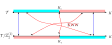
\includegraphics{z2latticephasestructure.pdf}
  \caption{$\Ztwo$格子ゲージ理論の相構造の図。}
  \label{fig:z2latticephasestructure}
\end{figure}

2次元Isingの場合と異なるところは、相転移の次数です。2次元Ising模型の相転移は二次相転移でしたが、$\Ztwo$格子ゲージ理論の相転移は一次相転移です。これは昔Creutzが数値計算により発見したものです。相転移が一次ですから、相転移点直上でもギャップがある理論になっているので、この相転移点を利用してトポロジカルでない連続理論を作ることはできません。

$K=K_c$のときには、$\Tcal$と$\Tcal/\Zb_{2}^{(1)}$は同じ理論になります。このとき、2次元の場合と同様にして半空間ゲージ化によりトポロジカル欠陥「双対性欠陥」を作ることができます。こうしてできる双対性欠陥は余次元1で、中心対称性の欠陥$\Zb_{2}^{(1)}$と合わせて様々な演算ができます。特に双対性欠陥の量子次元に当たる量($S^3$の分配関数)は$1/\sqrt{2}$になります。このことから双対性欠陥が非可逆であることが分かります。

\section{Maxwell理論}



\end{document}